\documentclass[12pt]{article}
\usepackage{parskip}
\usepackage{amsmath}
\usepackage{graphicx}
\usepackage{epstopdf}
\usepackage{cite}
\graphicspath{ {Images/} }

\begin{document}

\title{Diffusion 1D Simulator}
\author{Michelle King}

\begin{titlepage}
\maketitle
\end{titlepage}

\tableofcontents
\pagebreak

\section{Given Constants}
\[
n_{i}=1.5 \times 10^{10} cm^{-3}
\]

\section{Calculations}
\subsection{Built in Potential \cite[p. 222]{Pierret1996}}
Built in Potential \cite[eq. 5.10]{Pierret1996}
\begin{equation}
V_{bi} [eV]=\frac{k_{b} T}{q}log(\frac{N_{a}N_{d}}{ni^{2}})
\end{equation}

Know: 1 eV = e J and J/C = V

\begin{equation}
\frac{k_{b} T}{q} = 
\frac{k_{b} T [\frac{eV}{K}][K]}{e[C]}\frac{e[J]}{[eV]}=
\frac{k_{b} T [J]}{[C]}=
k_{b} T \ [V]
\end{equation}

For $V_{bi}$ in Volts:

\begin{equation}
V_{bi} [V]=k_{b} Tlog(\frac{N_{a}N_{d}}{ni^{2}})
\end{equation}

\subsection{Length of Device}

Distance from 0 to n equilibrium \cite[eq. 5.30a]{Pierret1996}
\[
K_{s} \ \epsilon_{0}=\epsilon
\]
\[
x_{n0}=\sqrt{\frac{2\epsilon}{q}\frac{N_{A}}{N_{D}(N_{A}+N_{D})}V_{bi}}
\]

Distance from 0 to p equilibrium \cite[eq. 5.30b]{Pierret1996}
\[
x_{p0}=\frac{N_{D} \ x_{n0}}{N_{A}}
\]

Width of Depletion Region is the the total distance from equilibrium to equilibrium.
\[
w_{0}=x_{n0}+x_{p0}
\]

Set the simulated device length proportional to the longest side
\[
x_{max}= Scale \times Max(x_{n0},x_{p0})
\]

\subsection{Mesh \cite[p. 36]{Vasileska2006}}
Mesh size must be smaller than the Intrinsic Debye Length \cite[eq. 3.12]{Vasileska2006}
\[
L_{di}=\sqrt{\frac{\epsilon k_{b} T}{n_{i} \ e^{2}}}
\]

Unit Analysis:
\[
L_{di}=\sqrt{\frac{\epsilon [\frac{F}{cm}] k_{b} T [eV]}{n_{i} [cm^{-3}] \ (e [C] * e ) }}
\]

\[
L_{di}=\sqrt{\frac{\epsilon [F] k_{b} T [V]}{n_{i} [cm^{-2}] \ e [C] }}
\]
\[
F=\frac{C}{V}
\]
\[
L_{di}=\sqrt{\frac{\epsilon k_{b} T}{n_{i}  \ e}[cm^{2}]}
\]

\[
L_{di}=\sqrt{\frac{\epsilon k_{b} T}{n_{i}  \ e}}[cm]
\]

Acceptor Extrinsic Debye Length 
\[
L_{da}=\sqrt{\frac{\epsilon k_{b} T}{N_{a} \ e^{2}}}
\]
\[
L_{da}=\sqrt{\frac{\epsilon k_{b} T}{N_{a} \ e}}[cm]
\]

Donor Extrinsic Debye Length 
\[
L_{dd}=\sqrt{\frac{\epsilon k_{b} T}{N_{d} \ e^{2}}}
\]
\[
L_{dd}=\sqrt{\frac{\epsilon k_{b} T}{N_{d} \ e}}[cm]
\]

Calculate dx as Minimum Extrinsic Debye Length
\[
dx= Scale \ Factor \times Minimum(Lda, Ldd)
\]

Scale Factor $<$ 1 acts as a scale factor to further refine the mesh

Set the total number of array points in the mesh
\[
n_{max}=int(\frac{x_{max}}{dx})
\]

\subsection{Doping Profile}
From points 1 to nmax/2,
\[
dop(i)=\frac{-N_{a}}{ni}
\]

From points nmax/2 to nmax,
\[
dop(i)=\frac{N_{d}}{ni}
\]

\subsection{Electric Field}
\[
E(x)=-\frac{d \psi}{dx}
\]
\[
E(i)=\frac{\psi_{i}-\psi_{i}+1}{dx}
\]

\subsection{Carrier Density}

\[
density(i)=p(i)-n(i)-dop(i)
\]

\subsection{Conduction Band Energy}
\[
E_{CB}(i)=0.5E_{g}-k_{b}T*psi(i)
\]

\section{Ohmic Contacts \cite[p. 3-23]{Software1998}}
"Ohmic contacts are implemented as simple Dirichlet boundary conditions where surface potential, electron concentration, and hole concentrations $(\psi_{s},n_{s},p_{s})$ are fixed. Minority and majority carier quasi-Fermi potentials are equal to the applied bias of the electrode, i.e. $ \phi_{n}=\phi_{p}=V_{applied}$. The potential $\psi_{s}$ is fixed at a value that is consistent with space charge neutrality, i.e."
\begin{equation}
	n_{s}+N_{A}^{-}=p_{s}+N_{D}^{+}
\end{equation}

"Equation can be solved for $\psi_{s},n_{s},p_{s},$ since $ \phi_{n},\phi_{p},$ are known. If Boltzmann statistics are used, substitution of equations yields:"
\begin{equation}
n_{s}=\frac{1}{2}[(N_{D}^{+}-N_{A}^{-})+\sqrt{(N_{D}^{+}-N_{A}^{-})^{2}+4n_{ie}^{2}}]
\end{equation}
\begin{equation}
p_{s}=\frac{n_{ie}^{2}}{n_{s}}
\end{equation}
\begin{equation}
\psi_{s}=\phi_{n}+\frac{kT_{L}}{q}\ln(\frac{n_{s}}{n_{ie}})=\phi_{p}-\frac{kT_{L}}{q}\ln(\frac{p}{n})
\end{equation}


\section{Gummel Method \cite[p. 40]{Vasileska2006}}
"Quasi-Linearization Procedure": \\
\\
1. "Choose an initial guess for the potential" $ \psi $
\\
\\
2. "Write the potential at the next iteration step as" $ \psi_{new} = \psi + \delta \psi $ "and substitute into the linear Poisson Equation"
\\
\\
3. "Use the linearization" $ exp(\pm \delta \psi) \approx 1 \pm \delta \psi $ "and discretize the resultant equation. This equation has a tridiagonal matrix form and is readily solved for" $ \delta \psi_{i} $
\\
\\
4. "Check for convergence. The residual... is calculated and convergence is achieved if the norm of the residual is smaller than a preset tolerance. If convergence is not achieved, return to step 2. In practice one might simply check the norm of the error"
\[\| \delta \psi \| \leq Tol \]


\section{Poisson Solver}

Linear Poisson Equation:

\begin{equation}
	\frac{\partial^{2} \psi}{\partial x^{2}} =
	-\frac{e}{\epsilon_{sc}}
	[p-n+N_{d}(x)-N_{a}(x)]
\end{equation}

where electron and hole density are defined as:
\begin{equation}
	n=n_{i}exp(\psi)
\end{equation}
\begin{equation}
	p=n_{i}exp(-\psi)
\end{equation}

This expands to:

\begin{equation}
	\frac{\partial^{2} \psi}{\partial x^{2}} =
	-\frac{e}{\epsilon_{sc}}
	[n_{i}exp(\psi)+n_{i}exp(-\psi)+\frac{N_{a}(x)-N_{d}(x)}{n_{i}}]
\end{equation}

Set $ \psi \rightarrow \psi + \delta $

The second derivative on the left side remains unchanged:

\begin{equation}
\frac{\partial^{2} \psi}{\partial x^{2}} 
\rightarrow
\frac{\partial^{2} (\psi + \delta \psi)}{\partial x^{2}} 
=
\frac{\partial^{2} \psi}{\partial x^{2}} +
\frac{\partial^{2} \delta \psi}{\partial x^{2}} 
=
\frac{\partial^{2} \psi}{\partial x^{2}}
\end{equation}

Substitute into the Linear Poisson Equation:

\begin{equation}
\frac{\partial^{2} \psi}{\partial x^{2}} =
-\frac{e}{\epsilon_{sc}}
[n_{i}exp(-\psi + \delta \psi)-n_{i}exp(\psi + \delta \psi)+N_{a}(x)-N_{d}(x)]
\end{equation}

Expand the exponentials:

\begin{equation}
\frac{\partial^{2} \psi}{\partial x^{2}} =
-\frac{e}{\epsilon_{sc}}
[n_{i}exp(-\psi)exp(\delta \psi)-n_{i}exp(\psi)exp(\delta \psi)+N_{a}(x)-N_{d}(x)]
\end{equation}

Assume: $ exp(\delta \psi) = 1 + \delta \psi$

\begin{equation}
\frac{\partial^{2} \psi}{\partial x^{2}} =
-\frac{e}{\epsilon_{sc}}
[n_{i}exp(-\psi)-n_{i}exp(\psi)+N_{a}(x)-N_{d}(x)]+
\delta \psi [n_{i}exp(-\psi)-n_{i}exp(\psi)]
\end{equation}

Reduce to original terms:

\begin{equation}
\frac{\partial^{2} \psi}{\partial x^{2}}
=
-\frac{e}{\epsilon_{sc}}
(p-n+C_{i})+\frac{e}{\epsilon_{sc}}\delta(p+n)
\end{equation}

Absorb factor of $ \frac{e}{\epsilon_{sc}} $ to reduce computation time:

\begin{equation}
\frac{\partial^{2} \psi}{\partial x^{2}}
=
(p-n+C_{i})+\delta(p+n)
\end{equation}


Finite Difference Scheme:

\begin{equation}
f''(x_{0})=\frac{f(x_{0}+\delta x)-2f(x_{0})+f(x_{0}-\delta x)}{\delta x^{2}}
\end{equation}
Finite Difference in Terms of Mesh Points:
\begin{equation}
\frac{\partial^{2} \psi}{\partial x^{2}}
=
\frac{
\psi^{n+1}_{i+1}-
2\psi^{n+1}_{i}+
\psi^{n+1}_{i-1}
}{\Delta^{2}}
\end{equation}


Finite Difference Representation of Linear Poisson Equation:
\begin{equation}
	\underbrace{\frac{1}{\Delta^{2}}}_{b_{i}}\psi^{n+1}_{i+1}
	-\underbrace{(\frac{2}{\Delta^{2}}+n_{i}+p_{i})}_{a_{i}}\psi^{n+1}_{i}
	+\underbrace{\frac{1}{\Delta^{2}}}_{c_{i}}\psi^{n+1}_{i-1}=
	-(p_{i}-n_{i}+C_{i})-(p_{i}+n_{i})\psi^{n}_{i}
\end{equation}

\begin{equation}
	=-(exp(-\psi_{i})-exp(\psi_{i})+dop_{i})-(exp(-\psi_{i})+exp(\psi_{i}))\psi^{n}_{i}
\end{equation}

\begin{equation}
	=exp(\psi_{i})-exp(-\psi_{i})-dop_{i}-(exp(-\psi_{i})+exp(\psi_{i}))\psi^{n}_{i}
\end{equation}

\section{LU Decomposition}
\subsection{Derivation}
Begin with a matrix A and apply Ohmic boundary conditions: \\
\[
A=
\begin{bmatrix}
    a_{1} & c_{1} & \hdotsfor{2} & 0 \\
    b_{2} & a_{2} &  c_{2} & \hdotsfor{2}  \\
   \hdotsfor{5} \\
   \hdotsfor{2}  & b_{n-1} & a_{n-1} &  c_{n-1} \\
   0 & \hdotsfor{2}  & b_{n} & a_{n}
\end{bmatrix}
=
\underbrace{
\begin{bmatrix}
    1 & 0 & \hdotsfor{2} & 0 \\
    b_{2} & a_{2} &  c_{2} & \hdotsfor{2}  \\
   \hdotsfor{5} \\
   \hdotsfor{2}  & b_{n-1} & a_{n-1} &  c_{n-1} \\
   0 & \hdotsfor{2}  & 0 & 1
\end{bmatrix}}_{\text{Ohmic BC Applied}}
\]

A Matrix A can be separated into multiplied lower and upper triangular matrices

\[
A=LU
\]

\[
\underbrace{
\begin{bmatrix}
    a_{1} & c_{1} & \hdotsfor{2} & 0 \\
    b_{2} & a_{2} &  c_{2} & \hdotsfor{2}  \\
   \hdotsfor{5} \\
   \hdotsfor{2}  & b_{n-1} & a_{n-1} &  c_{n-1} \\
   0 & \hdotsfor{2}  & b_{n} & a_{n}
\end{bmatrix}}_{\text{Matrix A}}
=
\underbrace{
\begin{bmatrix}
    1 &  \hdotsfor{3} & 0  \\
   \beta_{2} & 1 &  \hdotsfor{3}  \\
   \dots & \beta_{3} & 1 &  \hdotsfor{2}  \\
   \hdotsfor{5} \\
   0 & \hdotsfor{2}  & \beta_{n} & 1
\end{bmatrix}}_{\text{Lower Triangular Matrix L}}
\underbrace{
\begin{bmatrix}
    \alpha_{1} & c_{1} & \hdotsfor{1} & 0 \\
    \dots & \alpha_{2} &  c_{2} & \hdotsfor{1}  \\
   \hdotsfor{4} \\
   \hdotsfor{2} & \alpha_{n-1} &  c_{n-1} \\
   0 & \hdotsfor{2} & \alpha_{n}
\end{bmatrix}}_{\text{Upper Triangular Matrix U}}
\]

\begin{math}
Ax=f \\
LUx=f \\
Ux=y \\
Ly=f \\
\end{math}

Find L \& U from A \\
\begin{math}
\alpha_{1}=a_{1} \\
\beta_{k}=\frac{b_{k}}{\alpha_{k-1}} \\
\alpha_{k}=a_{k}-\beta_{k}c_{k-1}
\end{math}

Forward \& Back Substitution \\
\begin{math}
g_{1}=f_{1} \\
g_{i}=f_{i}-\beta_{i}g_{i} \\
i = 2, 3, \dots, n \\ 
\\
x_{n}=\frac{g_{n}}{\alpha_{n}} \\
x_{i}=\frac{g_{i}-c_{i}x_{i+1}}{\alpha_{i}} \\
i = n-1, \dots, 2, 1
\end{math}

\subsection{Relation to Physics}
\[
A=
\begin{bmatrix}
    1 & 0 & \hdotsfor{2} & 0 \\
    b_{2} & a_{2} &  c_{2} & \hdotsfor{2}  \\
   \hdotsfor{5} \\
   \hdotsfor{2}  & b_{n-1} & a_{n-1} &  c_{n-1} \\
   0 & \hdotsfor{2}  & 0 & 1
\end{bmatrix}
\]
\[
x = 
\begin{bmatrix}
\psi_{1} \\
\psi_{2} \\
\vdots \\
\psi_{n} \\
\end{bmatrix}
\]
\[
f = 
\begin{bmatrix}
exp(\psi_{1})-exp(-\psi_{1})-dop_{1}-exp(\psi_{1})*(exp(\psi_{1})+exp(-\psi_{1})) \\
exp(\psi_{2})-exp(-\psi_{2})-dop_{2}-exp(\psi_{2})*(exp(\psi_{2})+exp(-\psi_{2})) \\
\vdots \\
exp(\psi_{n})-exp(-\psi_{n})-dop_{n}-exp(\psi_{n})*(exp(\psi_{n})+exp(-\psi_{n})) \\
\end{bmatrix}
\]

\section{SRH Concentation Dependent Lifetime Model \cite[p. 3-60 ]{Software1998}}
Shockley-Read-Hall Recombination Model

\subsection{Equation}
\begin{equation}
R_{SRH}=
\frac
{pn-n_{i}^{2}}
{\tau_{p}[n+n_{i}exp(\frac{ETRAP}{k T})]+
	\tau_{n}[p+n_{i}exp(\frac{-ETRAP}{k T})]}
\end{equation}

Assume that the difference between the trap energy level and intrinsic Fermi level, $ETRAP=0$, so that recombination can be simplified to:

\begin{equation}
R_{SRH}=
\frac
{pn-n_{i}^{2}}
{\tau_{p}[n+n_{i}]+
	\tau_{n}[p+n_{i}]}
\end{equation}

The definitions of electron and hole concentration are:
\begin{align}
n &= n_{i} exp(\psi_{i}^{n})
\\
p &= n_{i} exp(-\psi_{i}^{n})
\end{align}
For the calculations in our model, the factor for the intrinsic concentration is removed:
\begin{align}
n(i) &= exp(\psi_{i}^{n})
\\
p(i) &= exp(-\psi_{i}^{n})
\end{align}

Expands to:
\begin{equation}
R_{SRH}=
\frac
{(n_{i} exp(-\psi_{i}^{n}))(n_{i} exp(\psi_{i}^{n}))-n_{i}^{2}}
{\tau_{p}[(n_{i} exp( \psi_{i}^{n}))+n_{i}]+
	\tau_{n}[(n_{i} exp(-\psi_{i}^{n}))+n_{i}]}
\end{equation}

\begin{equation}
R_{SRH}=
\frac
{n_{i}^{2}(exp(-\psi_{i}^{n})exp(\psi_{i}^{n})-1)}
{n_{i}(\tau_{p}[exp( \psi_{i}^{n})+1]+
	\tau_{n}[exp(-\psi_{i}^{n})+1])}
\end{equation}

\begin{equation}
R_{SRH}=
\frac
{n_{i}(exp(-\psi_{i}^{n})exp(\psi_{i}^{n})-1)}
{\tau_{p}[exp( \psi_{i}^{n})+1]+
	\tau_{n}[exp(-\psi_{i}^{n})+1]}
\end{equation}

\begin{equation}
R_{SRH}=
\frac
{n_{i}(p(i)n(i))-1)}
{\tau_{p}[n(i)+1]+
	\tau_{n}[p(i)+1]}
\end{equation}

\begin{equation}
\tau_{n}=\frac{TAUN0}{1+N/(NSRHN)}
\end{equation}

\begin{equation}
\tau_{p}=\frac{TAUP0}{1+N/(NSRHP)}
\end{equation}


\begin{center}
	\begin{tabular}{ |p{3cm}|p{3cm}|p{3cm}| }
		\hline
		\multicolumn{3}{|c|}{Parameters (Table 3-36 in Atlas)} \\
		\hline
		Parameter&Value&Units\\
		\hline
		TAUN0 & $1e-7$ & $s$\\
		NSRHN & $5e16$ & $cm^{-3}$\\
		TAUP0 & $1e-7$ & $s$\\
		NSRHP & $5e16$ & $cm^{-3}$\\
		\hline
	\end{tabular}
\end{center}

\subsection{Units}
\begin{equation}
\tau=\frac{TAU0 \ [s]}{1+N [cm^{-3}] /(NSRH [cm^{-3}])}
\end{equation}
\begin{equation}
\tau=\frac{TAU0 \ [s]}{1+N/(NSRH)}
\end{equation}

This leaves us with $ \tau $ in seconds, which is what we expect

\begin{equation}
R_{SRH}=
\frac
{pn [cm^{-6}] -n_{i}^{2}[cm^{-6}]}
{\tau_{p} [s] [n+n_{i}] [cm^{-3}]+
 \tau_{n} [s] [p+n_{i}] [cm^{-3}]}
\end{equation}

\begin{equation}
R_{SRH}=
\frac
{pn [cm^{-3}] -n_{i}^{2}[cm^{-3}]}
{\tau_{p} [s] [n+n_{i}] +
	\tau_{n} [s] [p+n_{i}]}
\end{equation}

This leaves us with $ R_{SRH} $ in units of [$cm^{-3}$/sec]

Since this number is with respect to real space and not the mesh, 

\section{The Arora Model for Low Field Mobility \cite[p. 3-35]{Software1998}}
\[
\mu_{n0}=
\mu_{1n}(\frac{T_{L}}{300})^{\alpha_{n}}+
\frac{\mu_{2n}(\frac{T_{L}}{300})^{\beta_{n}}}
{1+
\frac{N}
{N_{critn}(\frac{T_{L}}{300})^{\gamma_{n}}}}
\]

\[
\mu_{p0}=
\mu_{1p}(\frac{T_{L}}{300})^{\alpha_{p}}+
\frac{\mu_{2p}(\frac{T_{L}}{300})^{\beta_{p}}}
{1+
	\frac{N}
	{N_{critp}(\frac{T_{L}}{300})^{\gamma_{p}}}}
\]


\begin{center}
	\begin{tabular}{ |p{3cm}|p{3cm}|p{3cm}| }
		\hline
		\multicolumn{3}{|c|}{Parameters (Table 3-19 in Atlas)} \\
		\hline
		Parameter&Value&Units\\
		\hline
		MU1N 	& $88$ 		& $cm^{2}/(Vs)$\\
		MU1P 	& $54.3$ 	& $cm^{2}/(Vs)$\\
		MU2N 	& $1252.0$ 	& $cm^{2}/(Vs)$\\
		MU2P 	& $407.0$ 	& $cm^{2}/(Vs)$\\
		ALPHAN 	& $-0.57$ 	& $unitless$\\
		ALPHAP 	& $-0.57$ 	& $unitless$\\
		BETAN 	& $-2.33$	& $unitless$\\
		BETAP 	& $-2.23$	& $unitless$\\
		GAMMAN 	& $2.546$ 	& $unitless$\\
		GAMMAP 	& $2.546$ 	& $unitless$\\
		NCRITN 	& $1.43e17$ & $cm^{-3}$\\
		NCRITP 	& $2.67e17$ & $cm^{-3}$\\
		\hline
	\end{tabular}
\end{center}



\section{Field Dependent Mobility}

Field Dependent Mobility Model

\[
\mu(E)=\frac{\mu_{0}}{[1+(\frac{\mu_{0}E}{v_{sat}})^{\beta}]]^{1/\beta}}
\]

where 
\[
\beta = 
\begin{cases} 
1 & electrons\\
2 & holes
\end{cases}
\]

Saturation Velocity [cm/s]
\[
v_{sat}(T)=\frac{2.4*10^{7}}{1+0.8exp(\frac{T_{L}}{600})}
\]

but $ E(x)=-\frac{d\psi}{dx}$ so
\[
\mu(E)=\frac{\mu_{0}}{[1+(\frac{-\mu_{0}\frac{d\psi}{dx}}{v_{sat}})^{\beta}]]^{1/\beta}}
\]

We need to discretize this:
\[
\mu(E)=\frac{\mu_{0}}{[1+(\frac{-\mu_{0}\frac{\psi_{i+1}-\psi_{i}}{\Delta}}{v_{sat}})^{\beta}]]^{1/\beta}}
\]

\section{Diffusion From Mobility \cite{Pierret1996}}

Einstein Relation (Electrical mobility equation)

\[
D= \frac{k_{b}T}{q}\mu
\]



\section{Sharfetter-Gummel Discretization Scheme \cite[p.169]{Vasileska2006}}
\subsection{Discretize Current}
Current Equations
\begin{equation}
J_{n}=qn(x)\mu_{n}E(x)+qD_{n}\frac{dn}{dx}
\end{equation}
\begin{equation}
J_{p}=qp(x)\mu_{p}E(x)-qD_{p}\frac{dp}{dx}
\end{equation}

Continuity Equations
\begin{equation}
\frac{\partial n}{\partial t}=\frac{1}{q} \nabla \cdot \textbf{J}_{n}+U_{n}
\end{equation}
\begin{equation}
\frac{\partial p}{\partial t}=-\frac{1}{q} \nabla \cdot \textbf{J}_{p}+U_{p}
\end{equation}

Where $ U_{n} $ and $ U_{p} $ are the generation rates for electrons and holes respectively.

Put electric field in terms of potential in current equations
\begin{equation}
J_{n}=qn(x)\mu_{n}(-\frac{d\psi}{dx})+qD_{n}\frac{dn}{dx}
\end{equation}
\begin{equation}
J_{p}=qp(x)\mu_{p}(-\frac{d\psi}{dx})-qD_{p}\frac{dp}{dx}
\end{equation}

Discretize the Current Equations

\begin{equation}
J_{i+\frac{1}{2}}=
q\mu_{n}n_{i+\frac{1}{2}}(-\frac{\psi_{i+1}-\psi_{i}}{\Delta})+
qD_{n}\frac{n_{i+1}-n_{i}}{\Delta}
\end{equation}

\begin{equation}
J_{i+\frac{1}{2}}=
q\mu_{p}p_{i+\frac{1}{2}}(-\frac{\psi_{i+1}-\psi_{i}}{\Delta})-
qD_{p}\frac{p_{i+1}-p_{i}}{\Delta}
\end{equation}


Approximate $ n_{i+\frac{1}{2}} $ as an average of the two existing points around it.
\begin{equation}
n_{i+\frac{1}{2}}=\frac{n_{i+1}+n_{i}}{2}
\end{equation}

\begin{equation}
p_{i+\frac{1}{2}}=\frac{p_{i+1}+p_{i}}{2}
\end{equation}

Rewrite current equation
\begin{equation}
J_{i+\frac{1}{2}}=
n_{i+1}[-\frac{1}{2}q\mu_{n}(\frac{\psi_{i+1}-\psi_{i}}{\Delta})+q\frac{D_{n}}{\Delta}]-
n_{i}[\frac{1}{2}q\mu_{n}(\frac{\psi_{i+1}-\psi_{i}}{\Delta})+q\frac{D_{n}}{\Delta}]
\end{equation}

\begin{equation}
J_{i+\frac{1}{2}}=
-p_{i+1}[\frac{1}{2}q\mu_{p}(\frac{\psi_{i+1}-\psi_{i}}{\Delta})+q\frac{D_{p}}{\Delta}]+
p_{i}[-\frac{1}{2}q\mu_{p}(\frac{\psi_{i+1}-\psi_{i}}{\Delta})+q\frac{D_{p}}{\Delta}]
\end{equation}

\subsection{Solved Discretized Current}
The discretization of the continuity equation for electrons and holes is:
\begin{equation}
\frac{J_{i+\frac{1}{2}}-J_{i-\frac{1}{2}}}{\Delta}=q(R_{i}-G_{i})
\end{equation}
where R and G are Recombination and Generation Rates
\\
\\
Discretized J can be found by:
\begin{equation}
J_{i+\frac{1}{2}}=
q D_{i+\frac{1}{2}}
\frac
{n_{i+1}B(\psi'_{i+1}-\psi'_{i})-n_{i}B(\psi'_{i}-\psi'_{i+1})}
{\Delta}
\label{eqn:DiscCurrentElecEq}
\end{equation}
where
\begin{equation}
\psi'=\frac{q}{k_{b} T}\psi
\end{equation}
And
\begin{equation}
J_{i-\frac{1}{2}}=
q D_{i-\frac{1}{2}}
\frac
{n_{i}B(\psi'_{i}-\psi'_{i-1})-n_{i-1}B(\psi'_{i-1}-\psi'_{i})}
{\Delta}
\label{eqn:DiscCurrentHoleEq}
\end{equation}
This means that the equation we needs to solve turns into:
\begin{multline}
q D_{i+\frac{1}{2}}
\frac
{n_{i+1}B(\psi'_{i+1}-\psi'_{i})-n_{i}B(\psi'_{i}-\psi'_{i+1})}
{\Delta^{2}}-
\\
q D_{i-\frac{1}{2}}
\frac
{n_{i}B(\psi'_{i}-\psi'_{i-1})-n_{i-1}B(\psi'_{i-1}-\psi'_{i})}
{\Delta^{2}}=
q(R_{i}-G_{i})
\end{multline}
After the equation is divided by q, The left side of the equation can be sorted in terms of order of n:
\begin{multline}
\frac{D_{i-\frac{1}{2}}B(\psi'_{i-1}-\psi'_{i})}{{\Delta^{2}}}n_{i-1}-
\frac{D_{i+\frac{1}{2}}B(\psi'_{i}-\psi'_{i+1})+D_{i-\frac{1}{2}}B(\psi'_{i}-\psi'_{i-1})}{{\Delta^{2}}}n_{i}+
\\
\frac{D_{i+\frac{1}{2}}B(\psi'_{i+1}-\psi'_{i})}{{\Delta^{2}}}n_{i+1}
=R_{i}-G_{i}
\end{multline}
For LU Decomposition
\begin{align}
b(i)&=\frac{D_{i-\frac{1}{2}}B(\psi'_{i-1}-\psi'_{i})}{{\Delta^{2}}}
\\
a(i)&=-\frac{D_{i+\frac{1}{2}}B(\psi'_{i}-\psi'_{i+1})+D_{i-\frac{1}{2}}B(\psi'_{i}-\psi'_{i-1})}{{\Delta^{2}}}
\\
c(i)&=\frac{D_{i+\frac{1}{2}}B(\psi'_{i+1}-\psi'_{i})}{{\Delta^{2}}}
\\
x(i)&=n(i)
\\
f(i)&=R_{SRH}=
\frac
{n_{i}(p(i)n(i))-1)}
{\tau_{p}[n(i)+1]+
	\tau_{n}[p(i)+1]}
\end{align}



However, we treat n without the factor of the intrinsic concentration and only as a function of psi. This means the generation rate can be divided by ni for the calculation of n
\\
\\
D can also be approximated as an average of the closest values:
\begin{equation}
D_{i+\frac{1}{2}}=\frac{D_{i}+D_{i+1}}{2}
\label{eqn:DiffusionAvgEq+}
\end{equation}
\begin{equation}
D_{i-\frac{1}{2}}=\frac{D_{i}+D_{i-1}}{2}
\label{eqn:DiffusionAvgEq-}
\end{equation}


For LU Decomposition
\begin{align}
b(i)&=\frac{D_{i}+D_{i-1}}{2}\frac{B(\psi'_{i-1}-\psi'_{i})}{{\Delta^{2}}}
\\
a(i)&=
-(\frac{D_{i}+D_{i+1}}{2}\frac{
	B(\psi'_{i}-\psi'_{i+1})}{{\Delta^{2}}}
+\frac{D_{i}+D_{i-1}}{2}\frac{
	B(\psi'_{i}-\psi'_{i-1})}{{\Delta^{2}}})
\\
c(i)&=\frac{D_{i}+D_{i+1}}{2}\frac{B(\psi'_{i+1}-\psi'_{i})}{{\Delta^{2}}}
\\
x(i)&=n(i)
\\
f(i)&=R_{SRH}=
\frac
{n_{i}(p(i)n(i))-1)}
{\tau_{p}[n(i)+1]+
	\tau_{n}[p(i)+1]}
\end{align}

\section{Sharfetter-Gummel \cite[p.158-159] {Selberherr1984}}
These equations are changed from the book to fit the 1D Scheme. Also variables have been changed to make sense in context to the rest of these notes.
\subsection{Electrons}
\begin{multline}
D_{i+\frac{1}{2}}
\frac
{n_{i+1}B(\psi'_{i+1}-\psi'_{i})-n_{i}B(\psi'_{i}-\psi'_{i+1})}
{\Delta^{2}}-
\\
D_{i-\frac{1}{2}}
\frac
{n_{i}B(\psi'_{i}-\psi'_{i-1})-n_{i-1}B(\psi'_{i-1}-\psi'_{i})}
{\Delta^{2}}=
R_{i}
\end{multline}

\begin{multline}
n_{i+1}
\frac
{D_{i+\frac{1}{2}}B(\psi'_{i+1}-\psi'_{i})}
{\Delta^{2}}-
n_{i}
\frac{D_{i+\frac{1}{2}}B(\psi'_{i}-\psi'_{i+1})}
{\Delta^{2}}-
\\
n_{i}
\frac
{D_{i-\frac{1}{2}}B(\psi'_{i}-\psi'_{i-1})}
{\Delta^{2}}+
n_{i-1}	
\frac
{D_{i-\frac{1}{2}}B(\psi'_{i-1}-\psi'_{i})}
{\Delta^{2}}=
R_{i}
\end{multline}

\begin{multline}
n_{i+1}
\frac
{D_{i+\frac{1}{2}}B(\psi'_{i+1}-\psi'_{i})}
{\Delta^{2}}-
n_{i}
\frac
{D_{i+\frac{1}{2}}B(\psi'_{i}-\psi'_{i+1})+
D_{i-\frac{1}{2}}B(\psi'_{i}-\psi'_{i-1})}
{\Delta^{2}}+
\\
n_{i-1}	
\frac
{D_{i-\frac{1}{2}}B(\psi'_{i-1}-\psi'_{i})}
{\Delta^{2}}=
R_{i}
\end{multline}

\begin{align}
a(i)&=-\frac
{D_{i+\frac{1}{2}}B(\psi'_{i}-\psi'_{i+1})+
	D_{i-\frac{1}{2}}B(\psi'_{i}-\psi'_{i-1})}
{\Delta^{2}}
\\
b(i)&=\frac{D_{i-\frac{1}{2}}B(\psi'_{i-1}-\psi'_{i})}
{\Delta^{2}}
\\
c(i)&=\frac
{D_{i+\frac{1}{2}}B(\psi'_{i+1}-\psi'_{i})}
{\Delta^{2}}
\\
f(i)&=R_{i}
\end{align}

\subsection{Holes}
\begin{multline}
D_{i+\frac{1}{2}}
\frac
{p_{i+1}B(\psi'_{i}-\psi'_{i+1})-p_{i}B(\psi'_{i+1}-\psi'_{i})}
{\Delta^{2}}-
\\
D_{i-\frac{1}{2}}
\frac
{p_{i}B(\psi'_{i-1}-\psi'_{i})-p_{i-1}B(\psi'_{i}-\psi'_{i-1})}
{\Delta^{2}}=
R_{i}
\end{multline}

\begin{multline}
p_{i+1}
\frac
{D_{i+\frac{1}{2}}B(\psi'_{i}-\psi'_{i+1})}
{\Delta^{2}}-
p_{i}
\frac{D_{i+\frac{1}{2}}B(\psi'_{i+1}-\psi'_{i})}
{\Delta^{2}}-
\\
p_{i}
\frac
{D_{i-\frac{1}{2}}B(\psi'_{i-1}-\psi'_{i})}
{\Delta^{2}}+
p_{i-1}	
\frac
{D_{i-\frac{1}{2}}B(\psi'_{i}-\psi'_{i-1})}
{\Delta^{2}}=
R_{i}
\end{multline}

\begin{multline}
p_{i+1}
\frac
{D_{i+\frac{1}{2}}B(\psi'_{i}-\psi'_{i+1})}
{\Delta^{2}}-
p_{i}
\frac
{D_{i+\frac{1}{2}}B(\psi'_{i+1}-\psi'_{i})+
D_{i-\frac{1}{2}}B(\psi'_{i-1}-\psi'_{i})}
{\Delta^{2}}+
\\
p_{i-1}	
\frac
{D_{i-\frac{1}{2}}B(\psi'_{i}-\psi'_{i-1})}
{\Delta^{2}}=
R_{i}
\end{multline}

\begin{align}
a(i)&=-\frac
{D_{i+\frac{1}{2}}B(\psi'_{i+1}-\psi'_{i})+
	D_{i-\frac{1}{2}}B(\psi'_{i-1}-\psi'_{i})}
{\Delta^{2}}
\\
b(i)&=\frac
{D_{i-\frac{1}{2}}B(\psi'_{i}-\psi'_{i-1})}
{\Delta^{2}}
\\
c(i)&=\frac
{D_{i+\frac{1}{2}}B(\psi'_{i}-\psi'_{i+1})}
{\Delta^{2}}
\\
f(i)&=R_{i}
\end{align}

\section{Discretized Current Equations}
Using the discretized current equations eq. \ref{eqn:DiscCurrentElecEq} and eq. \ref{eqn:DiscCurrentHoleEq} and the discretized diffusion averages eq. \ref{eqn:DiffusionAvgEq+} and eq. \ref{eqn:DiffusionAvgEq-}:

\begin{equation}
J_{i+\frac{1}{2}}=
q \frac{D_{i}+D_{i+1}}{2}
\frac
{n_{i+1}B(\psi'_{i+1}-\psi'_{i})-n_{i}B(\psi'_{i}-\psi'_{i+1})}
{\Delta}
\end{equation}

\begin{equation}
J_{i-\frac{1}{2}}=
q \frac{D_{i}+D_{i-1}}{2}
\frac
{n_{i}B(\psi'_{i}-\psi'_{i-1})-n_{i-1}B(\psi'_{i-1}-\psi'_{i})}
{\Delta}
\end{equation}

\begin{equation}
J_{i}=\frac{J_{i-\frac{1}{2}}+J_{i+\frac{1}{2}}}{2}
\end{equation}

\begin{multline}
J_{i}=
\frac{q}
{2\Delta}
[\frac{D_{i}+D_{i+1}}{2}
(n_{i+1}B(\psi'_{i+1}-\psi'_{i})-n_{i}B(\psi'_{i}-\psi'_{i+1}))
+\\
\frac{D_{i}+D_{i-1}}{2}
(n_{i}B(\psi'_{i}-\psi'_{i-1})-n_{i-1}B(\psi'_{i-1}-\psi'_{i}))
]
\end{multline}

\begin{multline}
J_{i}=
\frac{q n_{i}}
{2\Delta}
[\frac{D_{i}+D_{i+1}}{2}
(n(i+1)B(\psi'_{i+1}-\psi'_{i})-n(i)B(\psi'_{i}-\psi'_{i+1}))
+\\
\frac{D_{i}+D_{i-1}}{2}
(n(i)B(\psi'_{i}-\psi'_{i-1})-n(i-1)B(\psi'_{i-1}-\psi'_{i}))
]
\end{multline}

\section{Bernoulli Function Implementation \cite[p.169] {Selberherr1984}}

Bernoulli Function:
\[
B(x)=\frac{x}{exp(x)-1}
\]

Suggested Implementation:
\[
B(x)=
\begin{cases} 
-x 							&         x	 \leq x1 \\
\frac{x}{exp(x)-1} 			& x1 \leq x  \leq x2 \\
1-\frac{x}{2} 				& x2 \leq x  \leq x3 \\
\frac{x exp(-x)}{1-exp(-x)} & x3 \leq x  \leq x4 \\
xexp(-x)					& x4 \leq x  \leq x5 \\
0							& x5 \leq x
\end{cases}
\]

Constants Discretely Defined by:
\begin{align}
exp(x1)-1&=-1
\\
x2/(exp(x2)-1)&=1-(x2/2), x2<0
\\
1-(x3/2)&=x3exp(-x3)/(1-exp(-x3)), x3>0
\\
1-exp(-x4)&=1
\\
exp(-x5)&=0
\end{align}

\section{Equilibrium Results}
\begin{figure}
    \centering
    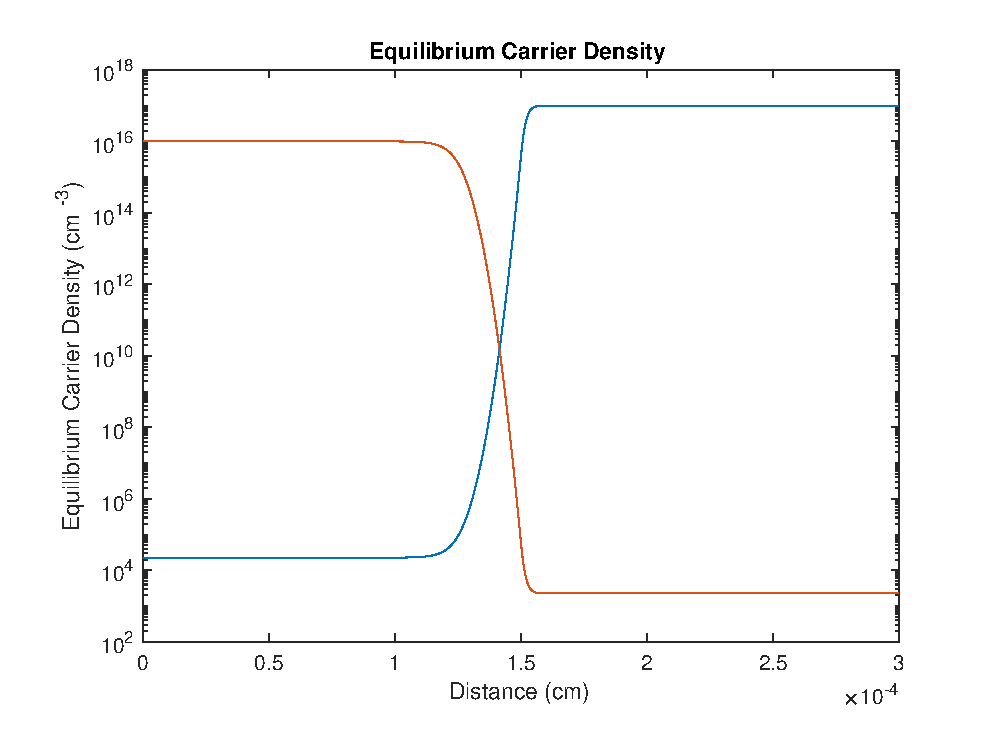
\includegraphics{EqCarrierDensity}
    \caption{Equilibrium Carrier Density}
\end{figure} 
\begin{figure}
    \centering
    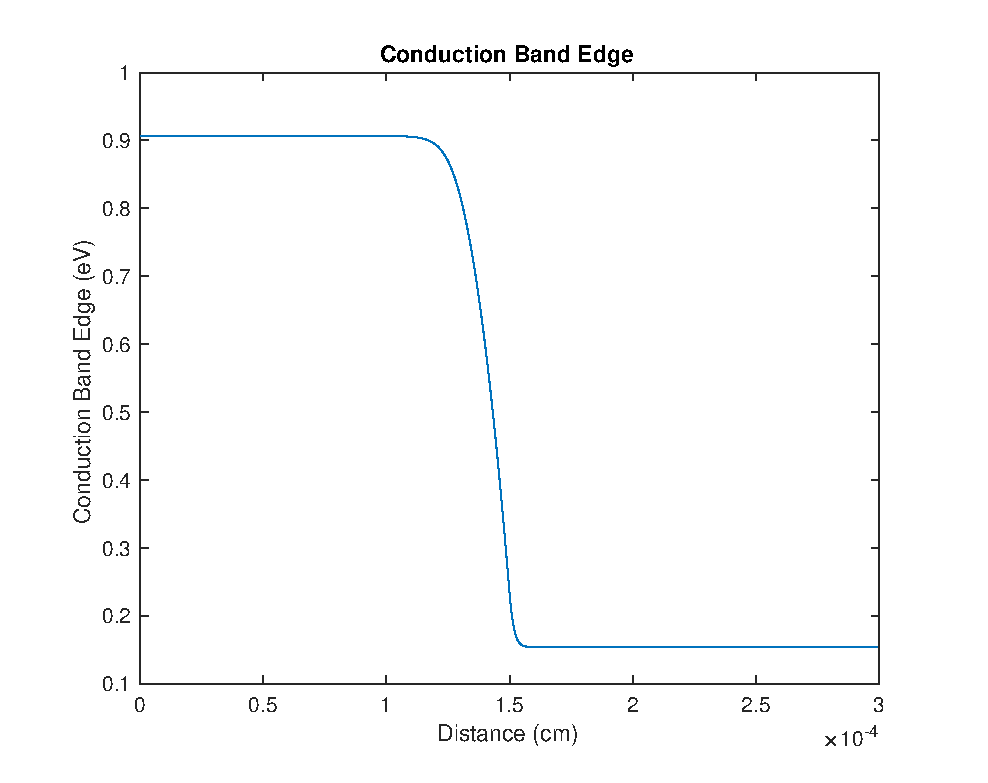
\includegraphics{EqConductionBandEdge}
    \caption{Equilibrium Carrier Density}
\end{figure} 

\begin{figure}
	\centering
	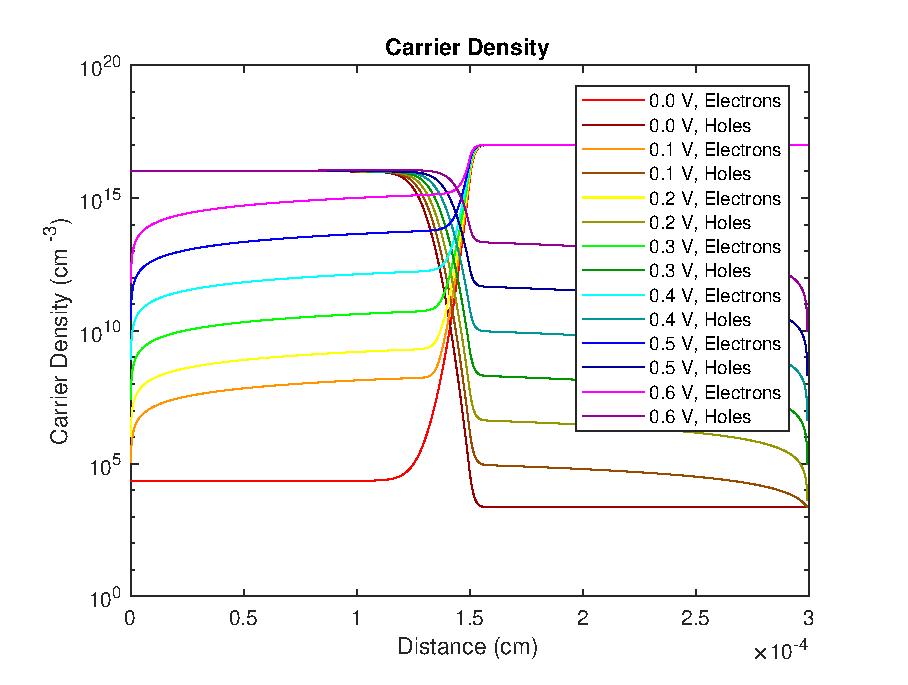
\includegraphics{CarrierDensityByVoltage}
	\caption{Carrier Density in a p-n junction by voltage steps of 0.1 V.}
\end{figure} 

\begin{figure}
	\centering
	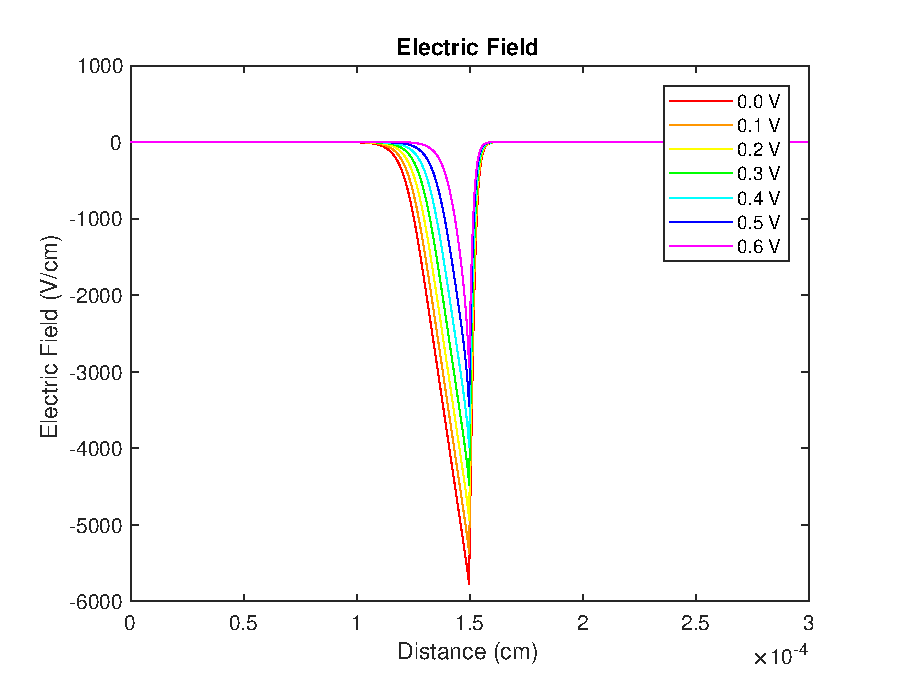
\includegraphics{ElectricFieldByVoltage}
	\caption{Electric Field in a p-n junction by voltage steps of 0.1 V. }
\end{figure} 

\begin{figure}
	\centering
	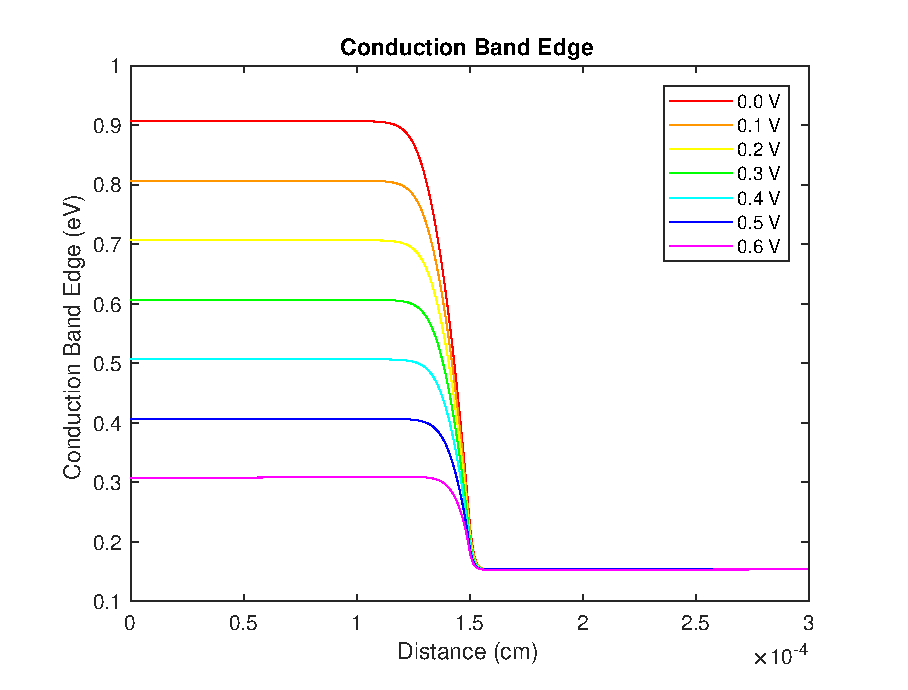
\includegraphics{CondBandEdgeByVoltage}
	\caption{Conduction Band in a p-n junction by voltage steps of 0.1 V. }
\end{figure} 

\begin{figure}
	\centering
	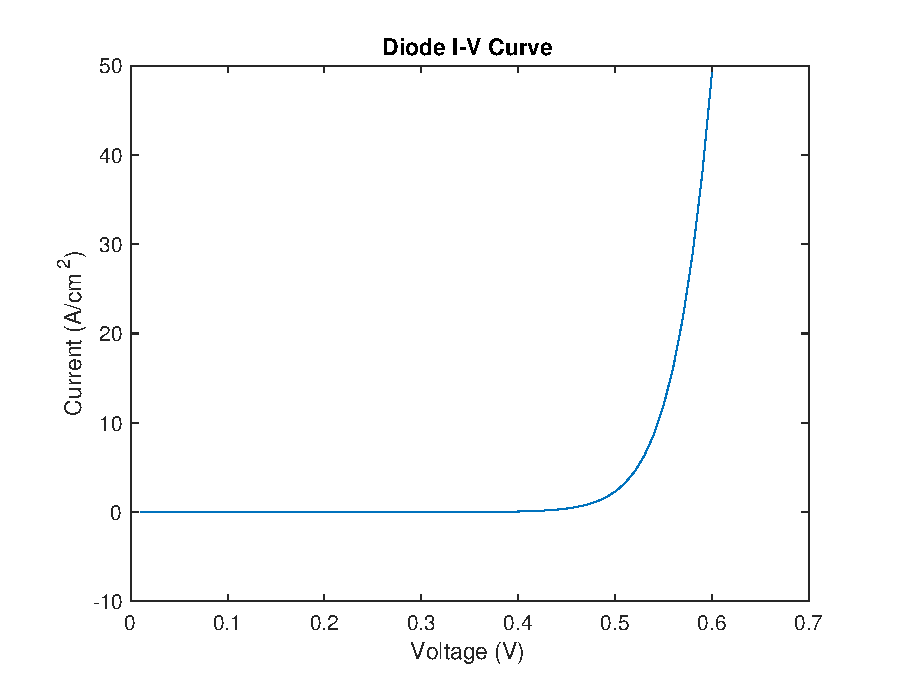
\includegraphics{DiodeIV}
	\caption{Diode IV Curve - Magnitude seems high?}
\end{figure} 

\bibliography{/Users/michelleking/GoogleDrive/Mendeley/Bibtex/Drift-Diffusion.bib}
\bibliographystyle{plain}


\end{document}